\documentclass[10pt]{article}
\usepackage[margin=1.8cm]{geometry}
\usepackage[T1]{fontenc}
\usepackage{lmodern}
\usepackage{microtype}
\usepackage{booktabs}
\usepackage{enumitem}
\usepackage{titlesec}
\usepackage{graphicx}
\usepackage{float}
\usepackage[hidelinks]{hyperref}

\titlespacing*{\section}{0pt}{8pt}{2pt}
\titleformat*{\section}{\normalsize\bfseries}
\setlist{nosep,leftmargin=1.2em,itemsep=1pt}
\setlength{\parskip}{3pt}
\setlength{\parindent}{0pt}
\setlength{\abovecaptionskip}{3pt}

\title{\vspace{-1.5cm}\large\textbf{XBRL Leaderboard: Comparing Financial LLMs and Agents on XBRL Tasks}}
\author{\normalsize Dev Gaglani \quad Stavan Desai}
\date{}

\begin{document}
\maketitle
\vspace{-1.3cm}

\section{Research question and gap}
Every number in an SEC filing is tagged in XBRL with a US-GAAP concept. The group already has XBRL benchmarks
(FinTagging~[1], XBRL-Agent~[2], FinAuditing~[3]), but no public page that compares models on them; the Open FinLLM
Leaderboard~[4,5] has no XBRL tasks.

\textbf{Question:} \emph{How well do open LLMs and agents handle XBRL tasks, and do the rankings stay the same when the
scoring rule or tool setting changes?}

\section{Scope}
\begin{itemize}
\item \textbf{First task:} concept linking (FinTagging, public subset): match one number from a filing to the right
concept among 17{,}388 US-GAAP concepts.
\item \textbf{Next tasks:} XBRL-Agent financial calculation and terminology, then FinAuditing.
\item \textbf{Overlapping questions:} duplicates across datasets are merged and conflicting answers are excluded. For
the first task, 500 items become 484 scored items; every removed item is listed.
\end{itemize}

\section{Evaluation}
\begin{itemize}
\item \textbf{Models:} Qwen2.5-7B and Llama-3.1-8B (instruction-tuned), run locally (4-bit, 6\,GB GPU).
\item \textbf{Conditions:} no tools, and with tag search (the model chooses from 100 candidate concepts).
\item \textbf{Scoring:} exact match with the correct concept, with 95\% confidence intervals. Each task keeps its
original metric.
\item \textbf{Baselines:} the no-tools run. Published scores are shown separately, since they use a different test set.
\end{itemize}

\section{What is done: the first demo}
We built a working local page with real results for the first task (Figure~1). It has three parts:
\begin{itemize}
\item \textbf{Results:} accuracy of each model with and without tag search on the 484 items. With tag search, both
models get 75 of 484 right (15.5\%). Without tools, Llama-3.1-8B gets 8 (1.7\%) and Qwen2.5-7B gets 6 (1.2\%). For
reference, the FinTagging paper reports 18.3\% for GPT-4o and 9.1\% for Llama-3.1-8B on its full test set.
\item \textbf{Example answers:} one correct and one wrong answer from Qwen2.5-7B with tag search, showing the filing
row, the correct concept and the model's answer.
\item \textbf{Why models fail:} search puts the correct concept among the 100 candidates for only 171 of 484 items
(35.3\%), and even then each model picks it for 75 of those 171 (43.9\%).
\end{itemize}
Every number on the page is recomputed by a script from the saved model answers and checked against the raw data.
\begin{figure}[t]
\centering
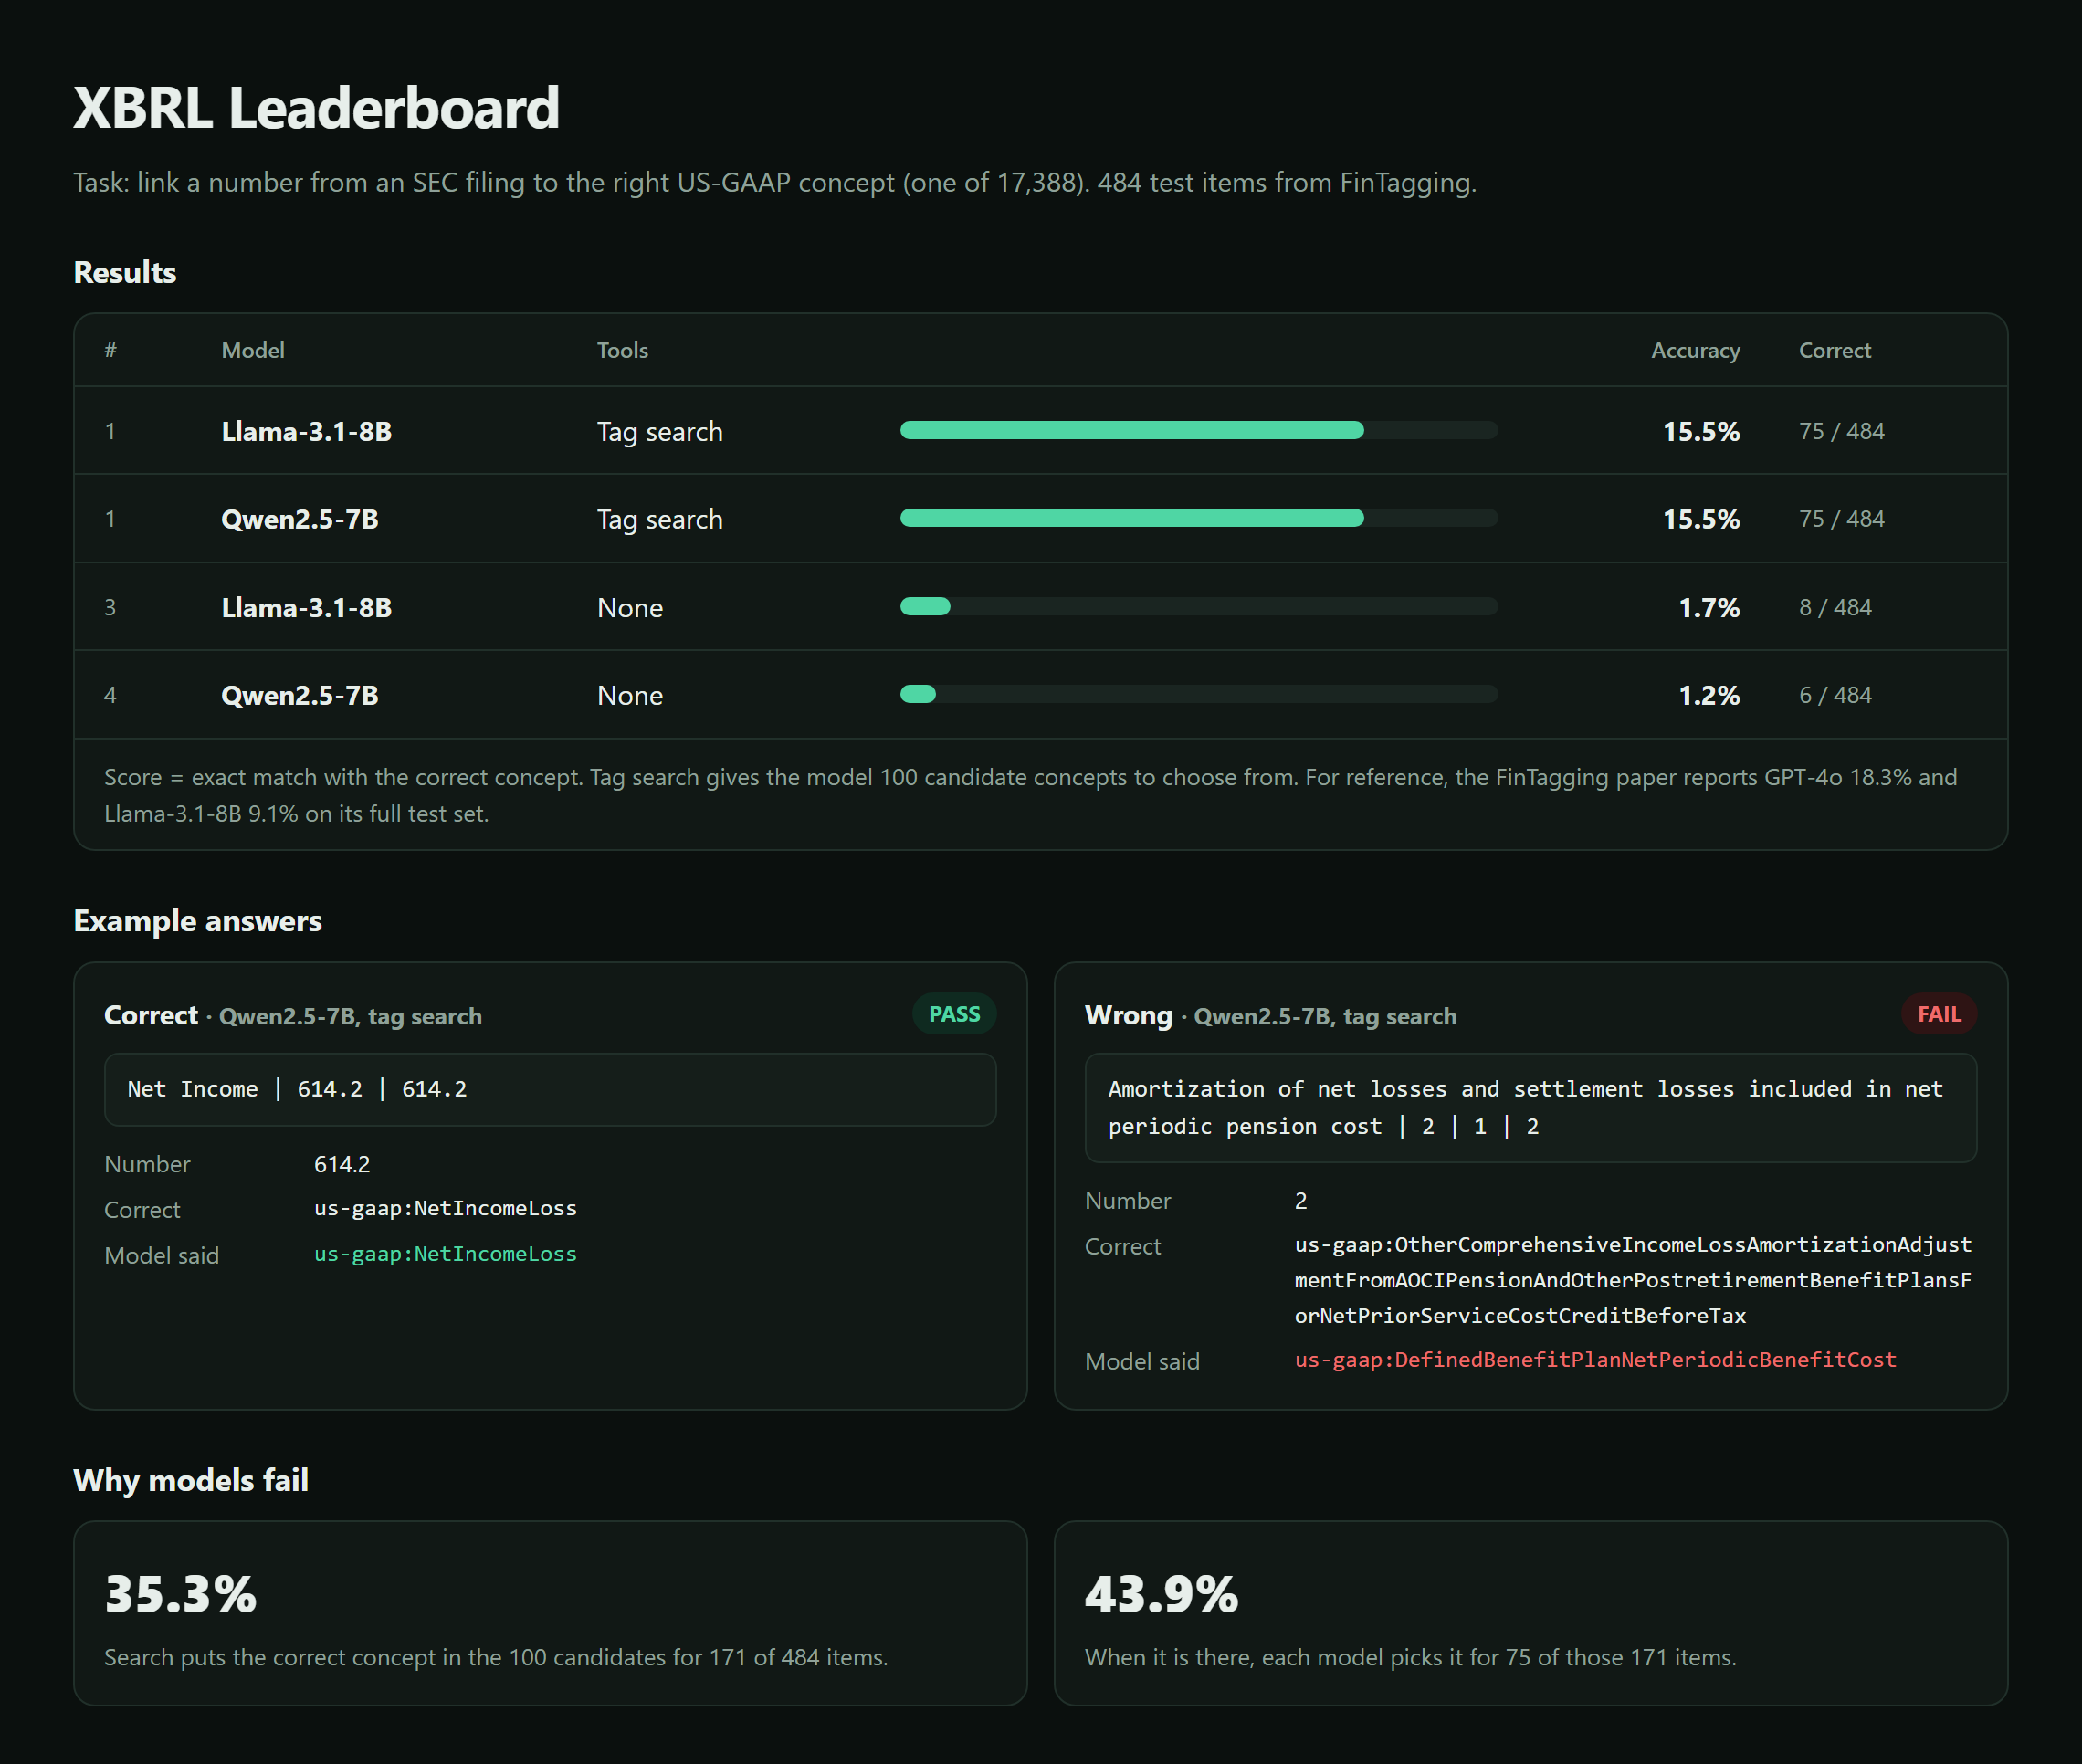
\includegraphics[width=0.75\textwidth]{demo_screenshot_v4.png}
\caption{\footnotesize The demo page: results table, one correct and one wrong answer, and why models fail.}
\end{figure}

\section{What we reuse and what we add}
\begin{itemize}
\item \textbf{Reuse:} the group's datasets and metrics, FinBen evaluation code~[6] where it fits, and the Open FinLLM
Leaderboard code (React interface, FastAPI backend, Hugging Face result storage).
\item \textbf{Add:} an XBRL page that shows, for each result, the dataset, model, tools, score and an example answer.
The leaderboard's task columns are currently hard-coded, so our first code change makes them configurable and adds a
tools field.
\end{itemize}

\section{Next steps and roles}
{\centering\small
\begin{tabular}{p{2.0cm}p{10.4cm}p{2.4cm}}
\toprule
When & Work & Lead \\
\midrule
Week 1   & Discuss the demo; agree the next task and where to host the page & Both \\
Weeks 2--3 & Add XBRL-Agent financial calculation for the same two models, with and without tools & Dev \\
Week 4   & Move the page onto the Open FinLLM Leaderboard code & Stavan \\
Weeks 5--6 & Check which rankings change under different scoring rules; short report & Both \\
\bottomrule
\end{tabular}\par}
\vspace{3pt}
Dev leads the evaluation; Stavan leads the page. We review results together.

\section{Where we need help}
\begin{itemize}
\item Access to FinTagging's full (gated) test set, to compare with published scores.
\item Which version of the group's evaluation code to use as the reference.
\item Where to host the page, and who reviews leaderboard changes.
\item Compute or API credits for models larger than 8B.
\end{itemize}

\vspace{4pt}
{\footnotesize\textbf{References.}
[1] Y.~Wang et al. FinTagging. arXiv:2505.20650, 2025.
[2] S.~Han et al. XBRL Agent. ICAIF, 2024.
[3] Y.~Wang et al. FinAuditing. arXiv:2510.08886, 2025.
[4] S.~C.~Lin et al. Open FinLLM Leaderboard: Towards financial AI readiness. arXiv:2501.10963, 2025.
[5] S.~Lin et al. Evaluation and benchmarking suite for financial LLMs and agents. arXiv:2602.19073, 2026.
[6] Q.~Xie et al. FinBen. arXiv:2402.12659, 2024.\par}
\end{document}
